\documentclass[twoside]{book}

% Packages required by doxygen
\usepackage{fixltx2e}
\usepackage{calc}
\usepackage{doxygen}
\usepackage[export]{adjustbox} % also loads graphicx
\usepackage{graphicx}
\usepackage[utf8]{inputenc}
\usepackage{makeidx}
\usepackage{multicol}
\usepackage{multirow}
\PassOptionsToPackage{warn}{textcomp}
\usepackage{textcomp}
\usepackage[nointegrals]{wasysym}
\usepackage[table]{xcolor}

% Font selection
\usepackage[T1]{fontenc}
\usepackage[scaled=.90]{helvet}
\usepackage{courier}
\usepackage{amssymb}
\usepackage{sectsty}
\renewcommand{\familydefault}{\sfdefault}
\allsectionsfont{%
  \fontseries{bc}\selectfont%
  \color{darkgray}%
}
\renewcommand{\DoxyLabelFont}{%
  \fontseries{bc}\selectfont%
  \color{darkgray}%
}
\newcommand{\+}{\discretionary{\mbox{\scriptsize$\hookleftarrow$}}{}{}}

% Page & text layout
\usepackage{geometry}
\geometry{%
  a4paper,%
  top=2.5cm,%
  bottom=2.5cm,%
  left=2.5cm,%
  right=2.5cm%
}
\tolerance=750
\hfuzz=15pt
\hbadness=750
\setlength{\emergencystretch}{15pt}
\setlength{\parindent}{0cm}
\setlength{\parskip}{3ex plus 2ex minus 2ex}
\makeatletter
\renewcommand{\paragraph}{%
  \@startsection{paragraph}{4}{0ex}{-1.0ex}{1.0ex}{%
    \normalfont\normalsize\bfseries\SS@parafont%
  }%
}
\renewcommand{\subparagraph}{%
  \@startsection{subparagraph}{5}{0ex}{-1.0ex}{1.0ex}{%
    \normalfont\normalsize\bfseries\SS@subparafont%
  }%
}
\makeatother

% Headers & footers
\usepackage{fancyhdr}
\pagestyle{fancyplain}
\fancyhead[LE]{\fancyplain{}{\bfseries\thepage}}
\fancyhead[CE]{\fancyplain{}{}}
\fancyhead[RE]{\fancyplain{}{\bfseries\leftmark}}
\fancyhead[LO]{\fancyplain{}{\bfseries\rightmark}}
\fancyhead[CO]{\fancyplain{}{}}
\fancyhead[RO]{\fancyplain{}{\bfseries\thepage}}
\fancyfoot[LE]{\fancyplain{}{}}
\fancyfoot[CE]{\fancyplain{}{}}
\fancyfoot[RE]{\fancyplain{}{\bfseries\scriptsize Generated by Doxygen }}
\fancyfoot[LO]{\fancyplain{}{\bfseries\scriptsize Generated by Doxygen }}
\fancyfoot[CO]{\fancyplain{}{}}
\fancyfoot[RO]{\fancyplain{}{}}
\renewcommand{\footrulewidth}{0.4pt}
\renewcommand{\chaptermark}[1]{%
  \markboth{#1}{}%
}
\renewcommand{\sectionmark}[1]{%
  \markright{\thesection\ #1}%
}

% Indices & bibliography
\usepackage{natbib}
\usepackage[titles]{tocloft}
\setcounter{tocdepth}{3}
\setcounter{secnumdepth}{5}
\makeindex

% Hyperlinks (required, but should be loaded last)
\usepackage{ifpdf}
\ifpdf
  \usepackage[pdftex,pagebackref=true]{hyperref}
\else
  \usepackage[ps2pdf,pagebackref=true]{hyperref}
\fi
\hypersetup{%
  colorlinks=true,%
  linkcolor=blue,%
  citecolor=blue,%
  unicode%
}

% Custom commands
\newcommand{\clearemptydoublepage}{%
  \newpage{\pagestyle{empty}\cleardoublepage}%
}

\usepackage{caption}
\captionsetup{labelsep=space,justification=centering,font={bf},singlelinecheck=off,skip=4pt,position=top}

%===== C O N T E N T S =====

\begin{document}

% Titlepage & ToC
\hypersetup{pageanchor=false,
             bookmarksnumbered=true,
             pdfencoding=unicode
            }
\pagenumbering{roman}
\begin{titlepage}
\vspace*{7cm}
\begin{center}%
{\Large My Project }\\
\vspace*{1cm}
{\large Generated by Doxygen 1.8.11}\\
\end{center}
\end{titlepage}
\clearemptydoublepage
\tableofcontents
\clearemptydoublepage
\pagenumbering{arabic}
\hypersetup{pageanchor=true}

%--- Begin generated contents ---
\chapter{Hierarchical Index}
\section{Class Hierarchy}
This inheritance list is sorted roughly, but not completely, alphabetically\+:\begin{DoxyCompactList}
\item \contentsline{section}{Fruit}{\pageref{classFruit}}{}
\begin{DoxyCompactList}
\item \contentsline{section}{Apple}{\pageref{classApple}}{}
\item \contentsline{section}{Grape}{\pageref{classGrape}}{}
\item \contentsline{section}{Orange}{\pageref{classOrange}}{}
\end{DoxyCompactList}
\item \contentsline{section}{List}{\pageref{classList}}{}
\item \contentsline{section}{List\+:\+:Node}{\pageref{structList_1_1Node}}{}
\end{DoxyCompactList}

\chapter{Class Index}
\section{Class List}
Here are the classes, structs, unions and interfaces with brief descriptions\+:\begin{DoxyCompactList}
\item\contentsline{section}{\hyperlink{structnode}{node} }{\pageref{structnode}}{}
\item\contentsline{section}{\hyperlink{structnode1}{node1} }{\pageref{structnode1}}{}
\item\contentsline{section}{\hyperlink{structnode__info}{node\+\_\+info} }{\pageref{structnode__info}}{}
\end{DoxyCompactList}

\chapter{File Index}
\section{File List}
Here is a list of all files with brief descriptions\+:\begin{DoxyCompactList}
\item\contentsline{section}{\hyperlink{Lab1_8c}{Lab1.\+c} }{\pageref{Lab1_8c}}{}
\end{DoxyCompactList}

\chapter{Class Documentation}
\hypertarget{classCar}{}\section{Car Class Reference}
\label{classCar}\index{Car@{Car}}


Inheritance diagram for Car\+:
\nopagebreak
\begin{figure}[H]
\begin{center}
\leavevmode
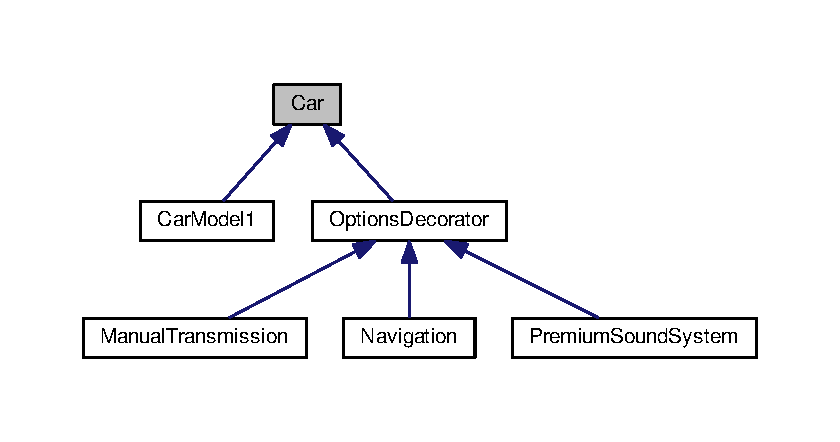
\includegraphics[width=350pt]{classCar__inherit__graph}
\end{center}
\end{figure}
\subsection*{Public Member Functions}
\begin{DoxyCompactItemize}
\item 
\hyperlink{classCar_a1c803f7c5038d3e31b368b0d0a35493c}{Car} ()
\item 
virtual string \hyperlink{classCar_a0d2f99b108e72e2a44360b38f16bbb46}{get\+Description} ()
\item 
virtual double \hyperlink{classCar_a7498766d25f7d4f15272f8055dd698f4}{get\+Cost} ()=0
\item 
virtual \hyperlink{classCar_a7f5f88d8a933b9de494e6beb818003f1}{$\sim$\+Car} ()
\end{DoxyCompactItemize}
\subsection*{Protected Attributes}
\begin{DoxyCompactItemize}
\item 
string \hyperlink{classCar_a2df6abd440445c77b48a45493245bb8e}{\+\_\+str}
\end{DoxyCompactItemize}


\subsection{Constructor \& Destructor Documentation}
\index{Car@{Car}!Car@{Car}}
\index{Car@{Car}!Car@{Car}}
\subsubsection[{\texorpdfstring{Car()}{Car()}}]{\setlength{\rightskip}{0pt plus 5cm}Car\+::\+Car (
\begin{DoxyParamCaption}
{}
\end{DoxyParamCaption}
)\hspace{0.3cm}{\ttfamily [inline]}}\hypertarget{classCar_a1c803f7c5038d3e31b368b0d0a35493c}{}\label{classCar_a1c803f7c5038d3e31b368b0d0a35493c}

\begin{DoxyCode}
11                 \{
12                         \hyperlink{classCar_a2df6abd440445c77b48a45493245bb8e}{\_str} = \textcolor{stringliteral}{"Unknown Car"};
13                 \}
\end{DoxyCode}
\index{Car@{Car}!````~Car@{$\sim$\+Car}}
\index{````~Car@{$\sim$\+Car}!Car@{Car}}
\subsubsection[{\texorpdfstring{$\sim$\+Car()}{~Car()}}]{\setlength{\rightskip}{0pt plus 5cm}virtual Car\+::$\sim$\+Car (
\begin{DoxyParamCaption}
{}
\end{DoxyParamCaption}
)\hspace{0.3cm}{\ttfamily [inline]}, {\ttfamily [virtual]}}\hypertarget{classCar_a7f5f88d8a933b9de494e6beb818003f1}{}\label{classCar_a7f5f88d8a933b9de494e6beb818003f1}

\begin{DoxyCode}
23                 \{
24                         cout << \textcolor{stringliteral}{"~Car()\(\backslash\)n"};
25                 \}
\end{DoxyCode}


\subsection{Member Function Documentation}
\index{Car@{Car}!get\+Cost@{get\+Cost}}
\index{get\+Cost@{get\+Cost}!Car@{Car}}
\subsubsection[{\texorpdfstring{get\+Cost()=0}{getCost()=0}}]{\setlength{\rightskip}{0pt plus 5cm}virtual double Car\+::get\+Cost (
\begin{DoxyParamCaption}
{}
\end{DoxyParamCaption}
)\hspace{0.3cm}{\ttfamily [pure virtual]}}\hypertarget{classCar_a7498766d25f7d4f15272f8055dd698f4}{}\label{classCar_a7498766d25f7d4f15272f8055dd698f4}


Implemented in \hyperlink{classManualTransmission_a33631e1b167a3aa7a2d86f5d8e2061bf}{Manual\+Transmission}, \hyperlink{classPremiumSoundSystem_ad14f7dae4adfb94572a80199174425af}{Premium\+Sound\+System}, \hyperlink{classNavigation_a2fedd3cf436e7487afc7a50d732d1054}{Navigation}, and \hyperlink{classCarModel1_aea624f25abb810c994dcd20f766418ed}{Car\+Model1}.

\index{Car@{Car}!get\+Description@{get\+Description}}
\index{get\+Description@{get\+Description}!Car@{Car}}
\subsubsection[{\texorpdfstring{get\+Description()}{getDescription()}}]{\setlength{\rightskip}{0pt plus 5cm}virtual string Car\+::get\+Description (
\begin{DoxyParamCaption}
{}
\end{DoxyParamCaption}
)\hspace{0.3cm}{\ttfamily [inline]}, {\ttfamily [virtual]}}\hypertarget{classCar_a0d2f99b108e72e2a44360b38f16bbb46}{}\label{classCar_a0d2f99b108e72e2a44360b38f16bbb46}


Reimplemented in \hyperlink{classManualTransmission_a3c5f0113936e6f8734a659ab8331a565}{Manual\+Transmission}, \hyperlink{classPremiumSoundSystem_a11267003bbf024bf19b811b0b28b22c1}{Premium\+Sound\+System}, \hyperlink{classNavigation_a2f7f7e9c43ecd76feabd46983b454e75}{Navigation}, and \hyperlink{classOptionsDecorator_a620341446534468345792530d454f76c}{Options\+Decorator}.


\begin{DoxyCode}
16                 \{       
17                         \textcolor{keywordflow}{return} \hyperlink{classCar_a2df6abd440445c77b48a45493245bb8e}{\_str};
18                 \}
\end{DoxyCode}


\subsection{Member Data Documentation}
\index{Car@{Car}!\+\_\+str@{\+\_\+str}}
\index{\+\_\+str@{\+\_\+str}!Car@{Car}}
\subsubsection[{\texorpdfstring{\+\_\+str}{_str}}]{\setlength{\rightskip}{0pt plus 5cm}string Car\+::\+\_\+str\hspace{0.3cm}{\ttfamily [protected]}}\hypertarget{classCar_a2df6abd440445c77b48a45493245bb8e}{}\label{classCar_a2df6abd440445c77b48a45493245bb8e}


The documentation for this class was generated from the following file\+:\begin{DoxyCompactItemize}
\item 
\hyperlink{Decorator_8cpp}{Decorator.\+cpp}\end{DoxyCompactItemize}

\hypertarget{classCarModel1}{}\section{Car\+Model1 Class Reference}
\label{classCarModel1}\index{Car\+Model1@{Car\+Model1}}


Inheritance diagram for Car\+Model1\+:
\nopagebreak
\begin{figure}[H]
\begin{center}
\leavevmode
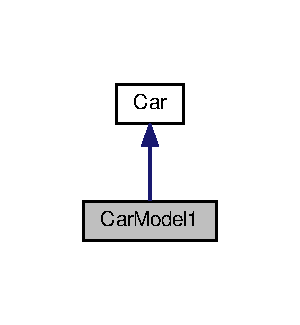
\includegraphics[width=144pt]{classCarModel1__inherit__graph}
\end{center}
\end{figure}


Collaboration diagram for Car\+Model1\+:
\nopagebreak
\begin{figure}[H]
\begin{center}
\leavevmode
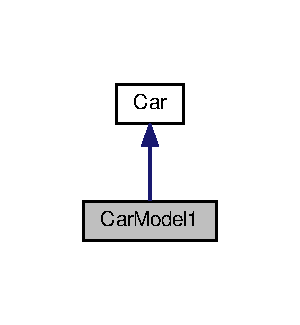
\includegraphics[width=144pt]{classCarModel1__coll__graph}
\end{center}
\end{figure}
\subsection*{Public Member Functions}
\begin{DoxyCompactItemize}
\item 
\hyperlink{classCarModel1_a197cba9e432896a0547ea1d488fe5b7f}{Car\+Model1} ()
\item 
virtual double \hyperlink{classCarModel1_aea624f25abb810c994dcd20f766418ed}{get\+Cost} ()
\item 
\hyperlink{classCarModel1_a77c7b74a972722e55d9990b56b7bc415}{$\sim$\+Car\+Model1} ()
\end{DoxyCompactItemize}
\subsection*{Additional Inherited Members}


\subsection{Constructor \& Destructor Documentation}
\index{Car\+Model1@{Car\+Model1}!Car\+Model1@{Car\+Model1}}
\index{Car\+Model1@{Car\+Model1}!Car\+Model1@{Car\+Model1}}
\subsubsection[{\texorpdfstring{Car\+Model1()}{CarModel1()}}]{\setlength{\rightskip}{0pt plus 5cm}Car\+Model1\+::\+Car\+Model1 (
\begin{DoxyParamCaption}
{}
\end{DoxyParamCaption}
)\hspace{0.3cm}{\ttfamily [inline]}}\hypertarget{classCarModel1_a197cba9e432896a0547ea1d488fe5b7f}{}\label{classCarModel1_a197cba9e432896a0547ea1d488fe5b7f}

\begin{DoxyCode}
44                 \{
45                         \hyperlink{classCar_a2df6abd440445c77b48a45493245bb8e}{\_str} = \textcolor{stringliteral}{"CarModel1"};
46                 \}
\end{DoxyCode}
\index{Car\+Model1@{Car\+Model1}!````~Car\+Model1@{$\sim$\+Car\+Model1}}
\index{````~Car\+Model1@{$\sim$\+Car\+Model1}!Car\+Model1@{Car\+Model1}}
\subsubsection[{\texorpdfstring{$\sim$\+Car\+Model1()}{~CarModel1()}}]{\setlength{\rightskip}{0pt plus 5cm}Car\+Model1\+::$\sim$\+Car\+Model1 (
\begin{DoxyParamCaption}
{}
\end{DoxyParamCaption}
)\hspace{0.3cm}{\ttfamily [inline]}}\hypertarget{classCarModel1_a77c7b74a972722e55d9990b56b7bc415}{}\label{classCarModel1_a77c7b74a972722e55d9990b56b7bc415}

\begin{DoxyCode}
53                 \{
54                         cout<<\textcolor{stringliteral}{"~CarModel1()\(\backslash\)n"};
55                 \}
\end{DoxyCode}


\subsection{Member Function Documentation}
\index{Car\+Model1@{Car\+Model1}!get\+Cost@{get\+Cost}}
\index{get\+Cost@{get\+Cost}!Car\+Model1@{Car\+Model1}}
\subsubsection[{\texorpdfstring{get\+Cost()}{getCost()}}]{\setlength{\rightskip}{0pt plus 5cm}virtual double Car\+Model1\+::get\+Cost (
\begin{DoxyParamCaption}
{}
\end{DoxyParamCaption}
)\hspace{0.3cm}{\ttfamily [inline]}, {\ttfamily [virtual]}}\hypertarget{classCarModel1_aea624f25abb810c994dcd20f766418ed}{}\label{classCarModel1_aea624f25abb810c994dcd20f766418ed}


Implements \hyperlink{classCar_a7498766d25f7d4f15272f8055dd698f4}{Car}.


\begin{DoxyCode}
48                 \{
49                         \textcolor{keywordflow}{return} 31000.23;
50                 \}
\end{DoxyCode}


The documentation for this class was generated from the following file\+:\begin{DoxyCompactItemize}
\item 
\hyperlink{Decorator_8cpp}{Decorator.\+cpp}\end{DoxyCompactItemize}

\hypertarget{classManualTransmission}{}\section{Manual\+Transmission Class Reference}
\label{classManualTransmission}\index{Manual\+Transmission@{Manual\+Transmission}}


Inheritance diagram for Manual\+Transmission\+:
\nopagebreak
\begin{figure}[H]
\begin{center}
\leavevmode
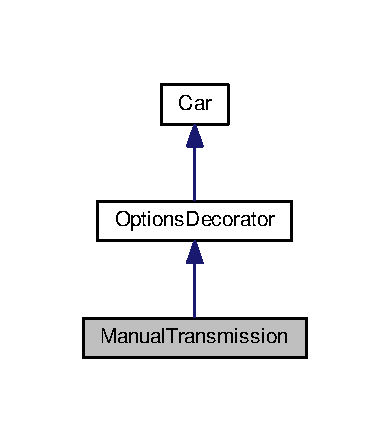
\includegraphics[width=187pt]{classManualTransmission__inherit__graph}
\end{center}
\end{figure}


Collaboration diagram for Manual\+Transmission\+:
\nopagebreak
\begin{figure}[H]
\begin{center}
\leavevmode
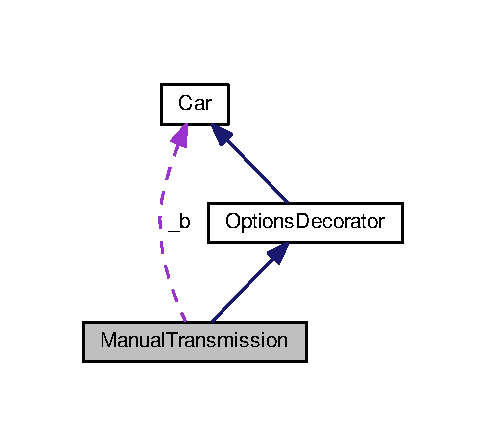
\includegraphics[width=233pt]{classManualTransmission__coll__graph}
\end{center}
\end{figure}
\subsection*{Public Member Functions}
\begin{DoxyCompactItemize}
\item 
\hyperlink{classManualTransmission_a5c4746be5cf077812d6d93e971129bbe}{Manual\+Transmission} (\hyperlink{classCar}{Car} $\ast$b)
\item 
string \hyperlink{classManualTransmission_a3c5f0113936e6f8734a659ab8331a565}{get\+Description} ()
\item 
double \hyperlink{classManualTransmission_a33631e1b167a3aa7a2d86f5d8e2061bf}{get\+Cost} ()
\item 
\hyperlink{classManualTransmission_a855eca38627c8eac4a546436f09727d7}{$\sim$\+Manual\+Transmission} ()
\end{DoxyCompactItemize}
\subsection*{Private Attributes}
\begin{DoxyCompactItemize}
\item 
\hyperlink{classCar}{Car} $\ast$ \hyperlink{classManualTransmission_ac32c597fb255d5ce8faeaf7d4a8525c2}{\+\_\+b}
\end{DoxyCompactItemize}
\subsection*{Additional Inherited Members}


\subsection{Constructor \& Destructor Documentation}
\index{Manual\+Transmission@{Manual\+Transmission}!Manual\+Transmission@{Manual\+Transmission}}
\index{Manual\+Transmission@{Manual\+Transmission}!Manual\+Transmission@{Manual\+Transmission}}
\subsubsection[{\texorpdfstring{Manual\+Transmission(\+Car $\ast$b)}{ManualTransmission(Car *b)}}]{\setlength{\rightskip}{0pt plus 5cm}Manual\+Transmission\+::\+Manual\+Transmission (
\begin{DoxyParamCaption}
\item[{{\bf Car} $\ast$}]{b}
\end{DoxyParamCaption}
)\hspace{0.3cm}{\ttfamily [inline]}}\hypertarget{classManualTransmission_a5c4746be5cf077812d6d93e971129bbe}{}\label{classManualTransmission_a5c4746be5cf077812d6d93e971129bbe}

\begin{DoxyCode}
112                 \{
113                         \hyperlink{classManualTransmission_ac32c597fb255d5ce8faeaf7d4a8525c2}{\_b} = b;
114                 \}
\end{DoxyCode}
\index{Manual\+Transmission@{Manual\+Transmission}!````~Manual\+Transmission@{$\sim$\+Manual\+Transmission}}
\index{````~Manual\+Transmission@{$\sim$\+Manual\+Transmission}!Manual\+Transmission@{Manual\+Transmission}}
\subsubsection[{\texorpdfstring{$\sim$\+Manual\+Transmission()}{~ManualTransmission()}}]{\setlength{\rightskip}{0pt plus 5cm}Manual\+Transmission\+::$\sim$\+Manual\+Transmission (
\begin{DoxyParamCaption}
{}
\end{DoxyParamCaption}
)\hspace{0.3cm}{\ttfamily [inline]}}\hypertarget{classManualTransmission_a855eca38627c8eac4a546436f09727d7}{}\label{classManualTransmission_a855eca38627c8eac4a546436f09727d7}

\begin{DoxyCode}
125                 \{
126                         cout << \textcolor{stringliteral}{"~ManualTransmission()\(\backslash\)n"};
127                         \textcolor{keyword}{delete} \hyperlink{classManualTransmission_ac32c597fb255d5ce8faeaf7d4a8525c2}{\_b};
128                 \}
\end{DoxyCode}


\subsection{Member Function Documentation}
\index{Manual\+Transmission@{Manual\+Transmission}!get\+Cost@{get\+Cost}}
\index{get\+Cost@{get\+Cost}!Manual\+Transmission@{Manual\+Transmission}}
\subsubsection[{\texorpdfstring{get\+Cost()}{getCost()}}]{\setlength{\rightskip}{0pt plus 5cm}double Manual\+Transmission\+::get\+Cost (
\begin{DoxyParamCaption}
{}
\end{DoxyParamCaption}
)\hspace{0.3cm}{\ttfamily [inline]}, {\ttfamily [virtual]}}\hypertarget{classManualTransmission_a33631e1b167a3aa7a2d86f5d8e2061bf}{}\label{classManualTransmission_a33631e1b167a3aa7a2d86f5d8e2061bf}


Implements \hyperlink{classCar_a7498766d25f7d4f15272f8055dd698f4}{Car}.


\begin{DoxyCode}
121                 \{
122                         \textcolor{keywordflow}{return} 0.30 + \hyperlink{classManualTransmission_ac32c597fb255d5ce8faeaf7d4a8525c2}{\_b}->\hyperlink{classCar_a7498766d25f7d4f15272f8055dd698f4}{getCost}();
123                 \}
\end{DoxyCode}


Here is the call graph for this function\+:
\nopagebreak
\begin{figure}[H]
\begin{center}
\leavevmode
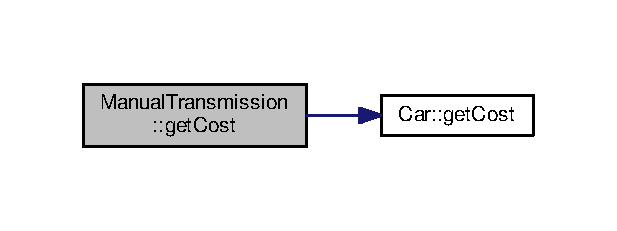
\includegraphics[width=296pt]{classManualTransmission_a33631e1b167a3aa7a2d86f5d8e2061bf_cgraph}
\end{center}
\end{figure}


\index{Manual\+Transmission@{Manual\+Transmission}!get\+Description@{get\+Description}}
\index{get\+Description@{get\+Description}!Manual\+Transmission@{Manual\+Transmission}}
\subsubsection[{\texorpdfstring{get\+Description()}{getDescription()}}]{\setlength{\rightskip}{0pt plus 5cm}string Manual\+Transmission\+::get\+Description (
\begin{DoxyParamCaption}
{}
\end{DoxyParamCaption}
)\hspace{0.3cm}{\ttfamily [inline]}, {\ttfamily [virtual]}}\hypertarget{classManualTransmission_a3c5f0113936e6f8734a659ab8331a565}{}\label{classManualTransmission_a3c5f0113936e6f8734a659ab8331a565}


Implements \hyperlink{classOptionsDecorator_a620341446534468345792530d454f76c}{Options\+Decorator}.


\begin{DoxyCode}
116                 \{
117                 \textcolor{keywordflow}{return} \hyperlink{classManualTransmission_ac32c597fb255d5ce8faeaf7d4a8525c2}{\_b}->\hyperlink{classCar_a0d2f99b108e72e2a44360b38f16bbb46}{getDescription}()+ \textcolor{stringliteral}{", ManualTransmission"};
118                 \}
\end{DoxyCode}


Here is the call graph for this function\+:
\nopagebreak
\begin{figure}[H]
\begin{center}
\leavevmode
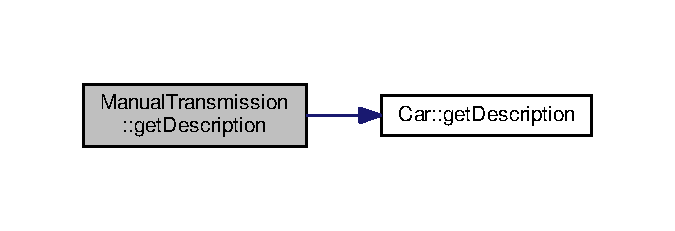
\includegraphics[width=324pt]{classManualTransmission_a3c5f0113936e6f8734a659ab8331a565_cgraph}
\end{center}
\end{figure}




\subsection{Member Data Documentation}
\index{Manual\+Transmission@{Manual\+Transmission}!\+\_\+b@{\+\_\+b}}
\index{\+\_\+b@{\+\_\+b}!Manual\+Transmission@{Manual\+Transmission}}
\subsubsection[{\texorpdfstring{\+\_\+b}{_b}}]{\setlength{\rightskip}{0pt plus 5cm}{\bf Car}$\ast$ Manual\+Transmission\+::\+\_\+b\hspace{0.3cm}{\ttfamily [private]}}\hypertarget{classManualTransmission_ac32c597fb255d5ce8faeaf7d4a8525c2}{}\label{classManualTransmission_ac32c597fb255d5ce8faeaf7d4a8525c2}


The documentation for this class was generated from the following file\+:\begin{DoxyCompactItemize}
\item 
\hyperlink{Decorator_8cpp}{Decorator.\+cpp}\end{DoxyCompactItemize}

\hypertarget{classNavigation}{}\section{Navigation Class Reference}
\label{classNavigation}\index{Navigation@{Navigation}}


Inheritance diagram for Navigation\+:
\nopagebreak
\begin{figure}[H]
\begin{center}
\leavevmode
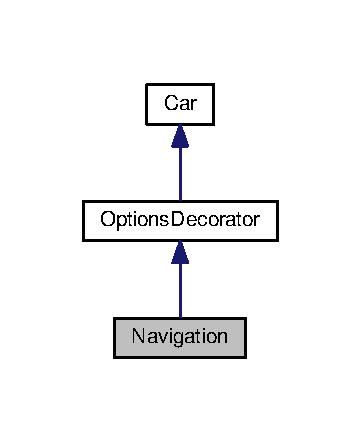
\includegraphics[width=173pt]{classNavigation__inherit__graph}
\end{center}
\end{figure}


Collaboration diagram for Navigation\+:
\nopagebreak
\begin{figure}[H]
\begin{center}
\leavevmode
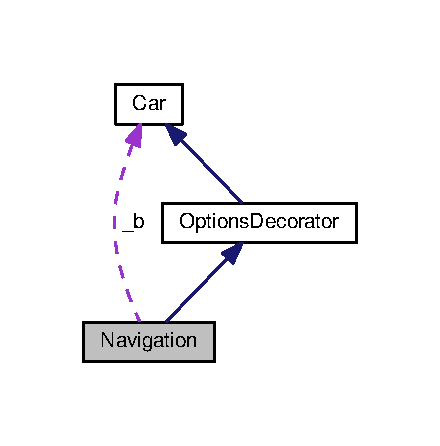
\includegraphics[width=211pt]{classNavigation__coll__graph}
\end{center}
\end{figure}
\subsection*{Public Member Functions}
\begin{DoxyCompactItemize}
\item 
\hyperlink{classNavigation_a99b76cf71edd512c71d7d9b01e2df464}{Navigation} (\hyperlink{classCar}{Car} $\ast$b)
\item 
string \hyperlink{classNavigation_a2f7f7e9c43ecd76feabd46983b454e75}{get\+Description} ()
\item 
double \hyperlink{classNavigation_a2fedd3cf436e7487afc7a50d732d1054}{get\+Cost} ()
\item 
\hyperlink{classNavigation_addd4022d716df48f4e55a1db69361ba7}{$\sim$\+Navigation} ()
\end{DoxyCompactItemize}
\subsection*{Private Attributes}
\begin{DoxyCompactItemize}
\item 
\hyperlink{classCar}{Car} $\ast$ \hyperlink{classNavigation_ae736423fb97d5b7993289d74e93aaff8}{\+\_\+b}
\end{DoxyCompactItemize}
\subsection*{Additional Inherited Members}


\subsection{Constructor \& Destructor Documentation}
\index{Navigation@{Navigation}!Navigation@{Navigation}}
\index{Navigation@{Navigation}!Navigation@{Navigation}}
\subsubsection[{\texorpdfstring{Navigation(\+Car $\ast$b)}{Navigation(Car *b)}}]{\setlength{\rightskip}{0pt plus 5cm}Navigation\+::\+Navigation (
\begin{DoxyParamCaption}
\item[{{\bf Car} $\ast$}]{b}
\end{DoxyParamCaption}
)\hspace{0.3cm}{\ttfamily [inline]}}\hypertarget{classNavigation_a99b76cf71edd512c71d7d9b01e2df464}{}\label{classNavigation_a99b76cf71edd512c71d7d9b01e2df464}

\begin{DoxyCode}
64                 \{
65                         \hyperlink{classNavigation_ae736423fb97d5b7993289d74e93aaff8}{\_b} = b;
66                 \}
\end{DoxyCode}
\index{Navigation@{Navigation}!````~Navigation@{$\sim$\+Navigation}}
\index{````~Navigation@{$\sim$\+Navigation}!Navigation@{Navigation}}
\subsubsection[{\texorpdfstring{$\sim$\+Navigation()}{~Navigation()}}]{\setlength{\rightskip}{0pt plus 5cm}Navigation\+::$\sim$\+Navigation (
\begin{DoxyParamCaption}
{}
\end{DoxyParamCaption}
)\hspace{0.3cm}{\ttfamily [inline]}}\hypertarget{classNavigation_addd4022d716df48f4e55a1db69361ba7}{}\label{classNavigation_addd4022d716df48f4e55a1db69361ba7}

\begin{DoxyCode}
77                 \{
78                         cout << \textcolor{stringliteral}{"~Navigation()\(\backslash\)n"};
79                         \textcolor{keyword}{delete} \hyperlink{classNavigation_ae736423fb97d5b7993289d74e93aaff8}{\_b};
80                 \}
\end{DoxyCode}


\subsection{Member Function Documentation}
\index{Navigation@{Navigation}!get\+Cost@{get\+Cost}}
\index{get\+Cost@{get\+Cost}!Navigation@{Navigation}}
\subsubsection[{\texorpdfstring{get\+Cost()}{getCost()}}]{\setlength{\rightskip}{0pt plus 5cm}double Navigation\+::get\+Cost (
\begin{DoxyParamCaption}
{}
\end{DoxyParamCaption}
)\hspace{0.3cm}{\ttfamily [inline]}, {\ttfamily [virtual]}}\hypertarget{classNavigation_a2fedd3cf436e7487afc7a50d732d1054}{}\label{classNavigation_a2fedd3cf436e7487afc7a50d732d1054}


Implements \hyperlink{classCar_a7498766d25f7d4f15272f8055dd698f4}{Car}.


\begin{DoxyCode}
73                 \{
74                         \textcolor{keywordflow}{return} 300.56 + \hyperlink{classNavigation_ae736423fb97d5b7993289d74e93aaff8}{\_b}->\hyperlink{classCar_a7498766d25f7d4f15272f8055dd698f4}{getCost}();
75                 \}
\end{DoxyCode}


Here is the call graph for this function\+:
\nopagebreak
\begin{figure}[H]
\begin{center}
\leavevmode
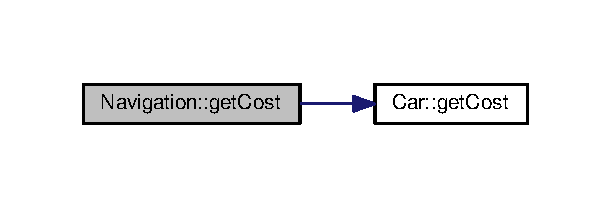
\includegraphics[width=293pt]{classNavigation_a2fedd3cf436e7487afc7a50d732d1054_cgraph}
\end{center}
\end{figure}


\index{Navigation@{Navigation}!get\+Description@{get\+Description}}
\index{get\+Description@{get\+Description}!Navigation@{Navigation}}
\subsubsection[{\texorpdfstring{get\+Description()}{getDescription()}}]{\setlength{\rightskip}{0pt plus 5cm}string Navigation\+::get\+Description (
\begin{DoxyParamCaption}
{}
\end{DoxyParamCaption}
)\hspace{0.3cm}{\ttfamily [inline]}, {\ttfamily [virtual]}}\hypertarget{classNavigation_a2f7f7e9c43ecd76feabd46983b454e75}{}\label{classNavigation_a2f7f7e9c43ecd76feabd46983b454e75}


Implements \hyperlink{classOptionsDecorator_a620341446534468345792530d454f76c}{Options\+Decorator}.


\begin{DoxyCode}
68                 \{
69                         \textcolor{keywordflow}{return} \hyperlink{classNavigation_ae736423fb97d5b7993289d74e93aaff8}{\_b}->\hyperlink{classCar_a0d2f99b108e72e2a44360b38f16bbb46}{getDescription}() + \textcolor{stringliteral}{", Navigation"};
70                 \}
\end{DoxyCode}


Here is the call graph for this function\+:
\nopagebreak
\begin{figure}[H]
\begin{center}
\leavevmode
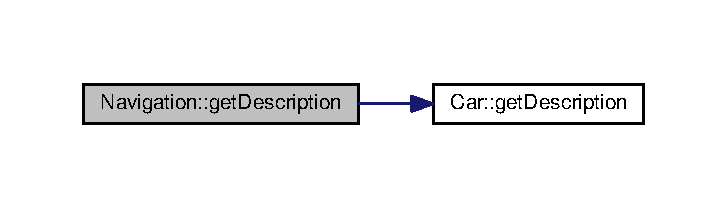
\includegraphics[width=349pt]{classNavigation_a2f7f7e9c43ecd76feabd46983b454e75_cgraph}
\end{center}
\end{figure}




\subsection{Member Data Documentation}
\index{Navigation@{Navigation}!\+\_\+b@{\+\_\+b}}
\index{\+\_\+b@{\+\_\+b}!Navigation@{Navigation}}
\subsubsection[{\texorpdfstring{\+\_\+b}{_b}}]{\setlength{\rightskip}{0pt plus 5cm}{\bf Car}$\ast$ Navigation\+::\+\_\+b\hspace{0.3cm}{\ttfamily [private]}}\hypertarget{classNavigation_ae736423fb97d5b7993289d74e93aaff8}{}\label{classNavigation_ae736423fb97d5b7993289d74e93aaff8}


The documentation for this class was generated from the following file\+:\begin{DoxyCompactItemize}
\item 
\hyperlink{Decorator_8cpp}{Decorator.\+cpp}\end{DoxyCompactItemize}

\hypertarget{classOptionsDecorator}{}\section{Options\+Decorator Class Reference}
\label{classOptionsDecorator}\index{Options\+Decorator@{Options\+Decorator}}


Inheritance diagram for Options\+Decorator\+:
\nopagebreak
\begin{figure}[H]
\begin{center}
\leavevmode
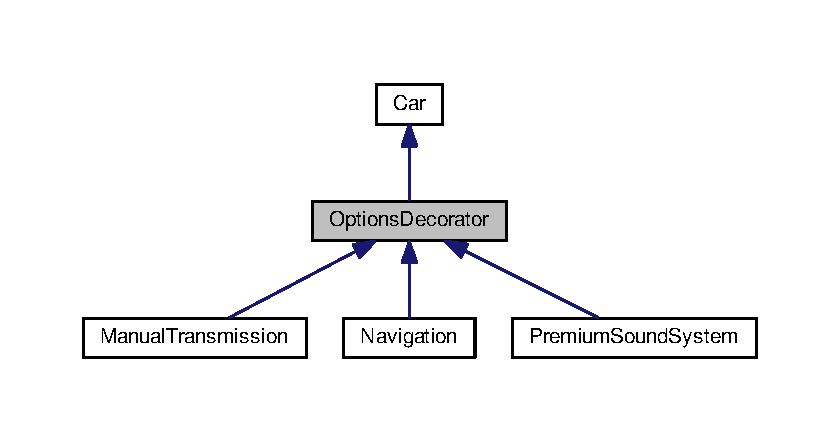
\includegraphics[width=350pt]{classOptionsDecorator__inherit__graph}
\end{center}
\end{figure}


Collaboration diagram for Options\+Decorator\+:
\nopagebreak
\begin{figure}[H]
\begin{center}
\leavevmode
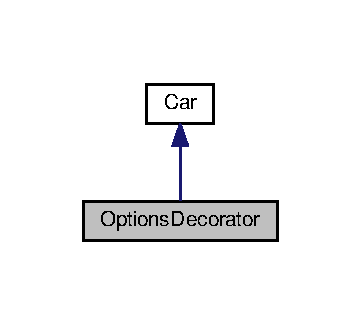
\includegraphics[width=173pt]{classOptionsDecorator__coll__graph}
\end{center}
\end{figure}
\subsection*{Public Member Functions}
\begin{DoxyCompactItemize}
\item 
virtual string \hyperlink{classOptionsDecorator_a620341446534468345792530d454f76c}{get\+Description} ()=0
\item 
virtual \hyperlink{classOptionsDecorator_a78a94ffd4dd252e91d63a859b24a6713}{$\sim$\+Options\+Decorator} ()
\end{DoxyCompactItemize}
\subsection*{Additional Inherited Members}


\subsection{Constructor \& Destructor Documentation}
\index{Options\+Decorator@{Options\+Decorator}!````~Options\+Decorator@{$\sim$\+Options\+Decorator}}
\index{````~Options\+Decorator@{$\sim$\+Options\+Decorator}!Options\+Decorator@{Options\+Decorator}}
\subsubsection[{\texorpdfstring{$\sim$\+Options\+Decorator()}{~OptionsDecorator()}}]{\setlength{\rightskip}{0pt plus 5cm}virtual Options\+Decorator\+::$\sim$\+Options\+Decorator (
\begin{DoxyParamCaption}
{}
\end{DoxyParamCaption}
)\hspace{0.3cm}{\ttfamily [inline]}, {\ttfamily [virtual]}}\hypertarget{classOptionsDecorator_a78a94ffd4dd252e91d63a859b24a6713}{}\label{classOptionsDecorator_a78a94ffd4dd252e91d63a859b24a6713}

\begin{DoxyCode}
34                 \{
35                         cout<<\textcolor{stringliteral}{"~OptionsDecorator()\(\backslash\)n"};
36                 \}
\end{DoxyCode}


\subsection{Member Function Documentation}
\index{Options\+Decorator@{Options\+Decorator}!get\+Description@{get\+Description}}
\index{get\+Description@{get\+Description}!Options\+Decorator@{Options\+Decorator}}
\subsubsection[{\texorpdfstring{get\+Description()=0}{getDescription()=0}}]{\setlength{\rightskip}{0pt plus 5cm}virtual string Options\+Decorator\+::get\+Description (
\begin{DoxyParamCaption}
{}
\end{DoxyParamCaption}
)\hspace{0.3cm}{\ttfamily [pure virtual]}}\hypertarget{classOptionsDecorator_a620341446534468345792530d454f76c}{}\label{classOptionsDecorator_a620341446534468345792530d454f76c}


Reimplemented from \hyperlink{classCar_a0d2f99b108e72e2a44360b38f16bbb46}{Car}.



Implemented in \hyperlink{classManualTransmission_a3c5f0113936e6f8734a659ab8331a565}{Manual\+Transmission}, \hyperlink{classPremiumSoundSystem_a11267003bbf024bf19b811b0b28b22c1}{Premium\+Sound\+System}, and \hyperlink{classNavigation_a2f7f7e9c43ecd76feabd46983b454e75}{Navigation}.



The documentation for this class was generated from the following file\+:\begin{DoxyCompactItemize}
\item 
\hyperlink{Decorator_8cpp}{Decorator.\+cpp}\end{DoxyCompactItemize}

\hypertarget{classPremiumSoundSystem}{}\section{Premium\+Sound\+System Class Reference}
\label{classPremiumSoundSystem}\index{Premium\+Sound\+System@{Premium\+Sound\+System}}


Inheritance diagram for Premium\+Sound\+System\+:
\nopagebreak
\begin{figure}[H]
\begin{center}
\leavevmode
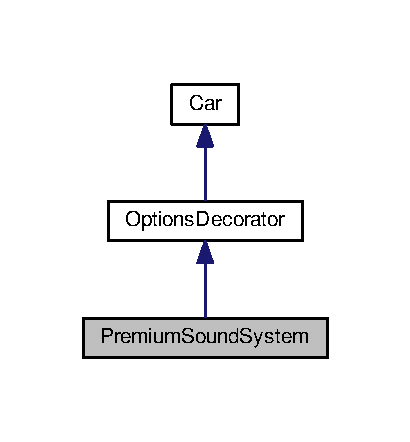
\includegraphics[width=197pt]{classPremiumSoundSystem__inherit__graph}
\end{center}
\end{figure}


Collaboration diagram for Premium\+Sound\+System\+:
\nopagebreak
\begin{figure}[H]
\begin{center}
\leavevmode
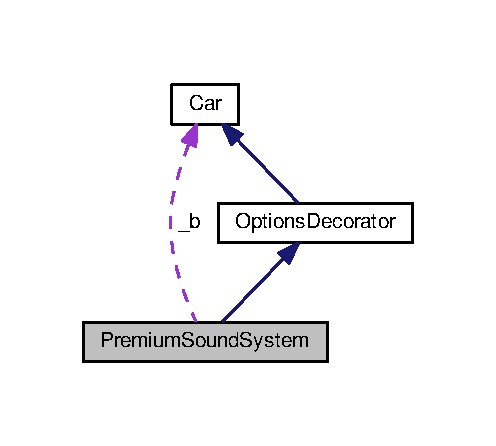
\includegraphics[width=238pt]{classPremiumSoundSystem__coll__graph}
\end{center}
\end{figure}
\subsection*{Public Member Functions}
\begin{DoxyCompactItemize}
\item 
\hyperlink{classPremiumSoundSystem_a8cbc764713229e2b97af1f8e0c95b7e8}{Premium\+Sound\+System} (\hyperlink{classCar}{Car} $\ast$b)
\item 
string \hyperlink{classPremiumSoundSystem_a11267003bbf024bf19b811b0b28b22c1}{get\+Description} ()
\item 
double \hyperlink{classPremiumSoundSystem_ad14f7dae4adfb94572a80199174425af}{get\+Cost} ()
\item 
\hyperlink{classPremiumSoundSystem_a249ed821c592d454328b2cf54fe9e2f3}{$\sim$\+Premium\+Sound\+System} ()
\end{DoxyCompactItemize}
\subsection*{Private Attributes}
\begin{DoxyCompactItemize}
\item 
\hyperlink{classCar}{Car} $\ast$ \hyperlink{classPremiumSoundSystem_a441bc8062467c6c45cd47bca4b8950dd}{\+\_\+b}
\end{DoxyCompactItemize}
\subsection*{Additional Inherited Members}


\subsection{Constructor \& Destructor Documentation}
\index{Premium\+Sound\+System@{Premium\+Sound\+System}!Premium\+Sound\+System@{Premium\+Sound\+System}}
\index{Premium\+Sound\+System@{Premium\+Sound\+System}!Premium\+Sound\+System@{Premium\+Sound\+System}}
\subsubsection[{\texorpdfstring{Premium\+Sound\+System(\+Car $\ast$b)}{PremiumSoundSystem(Car *b)}}]{\setlength{\rightskip}{0pt plus 5cm}Premium\+Sound\+System\+::\+Premium\+Sound\+System (
\begin{DoxyParamCaption}
\item[{{\bf Car} $\ast$}]{b}
\end{DoxyParamCaption}
)\hspace{0.3cm}{\ttfamily [inline]}}\hypertarget{classPremiumSoundSystem_a8cbc764713229e2b97af1f8e0c95b7e8}{}\label{classPremiumSoundSystem_a8cbc764713229e2b97af1f8e0c95b7e8}

\begin{DoxyCode}
88                 \{
89                         \hyperlink{classPremiumSoundSystem_a441bc8062467c6c45cd47bca4b8950dd}{\_b} = b;
90                 \}
\end{DoxyCode}
\index{Premium\+Sound\+System@{Premium\+Sound\+System}!````~Premium\+Sound\+System@{$\sim$\+Premium\+Sound\+System}}
\index{````~Premium\+Sound\+System@{$\sim$\+Premium\+Sound\+System}!Premium\+Sound\+System@{Premium\+Sound\+System}}
\subsubsection[{\texorpdfstring{$\sim$\+Premium\+Sound\+System()}{~PremiumSoundSystem()}}]{\setlength{\rightskip}{0pt plus 5cm}Premium\+Sound\+System\+::$\sim$\+Premium\+Sound\+System (
\begin{DoxyParamCaption}
{}
\end{DoxyParamCaption}
)\hspace{0.3cm}{\ttfamily [inline]}}\hypertarget{classPremiumSoundSystem_a249ed821c592d454328b2cf54fe9e2f3}{}\label{classPremiumSoundSystem_a249ed821c592d454328b2cf54fe9e2f3}

\begin{DoxyCode}
101                 \{
102                         cout << \textcolor{stringliteral}{"~PremiumSoundSystem()\(\backslash\)n"};
103                         \textcolor{keyword}{delete} \hyperlink{classPremiumSoundSystem_a441bc8062467c6c45cd47bca4b8950dd}{\_b};
104                 \}
\end{DoxyCode}


\subsection{Member Function Documentation}
\index{Premium\+Sound\+System@{Premium\+Sound\+System}!get\+Cost@{get\+Cost}}
\index{get\+Cost@{get\+Cost}!Premium\+Sound\+System@{Premium\+Sound\+System}}
\subsubsection[{\texorpdfstring{get\+Cost()}{getCost()}}]{\setlength{\rightskip}{0pt plus 5cm}double Premium\+Sound\+System\+::get\+Cost (
\begin{DoxyParamCaption}
{}
\end{DoxyParamCaption}
)\hspace{0.3cm}{\ttfamily [inline]}, {\ttfamily [virtual]}}\hypertarget{classPremiumSoundSystem_ad14f7dae4adfb94572a80199174425af}{}\label{classPremiumSoundSystem_ad14f7dae4adfb94572a80199174425af}


Implements \hyperlink{classCar_a7498766d25f7d4f15272f8055dd698f4}{Car}.


\begin{DoxyCode}
97                 \{
98                         \textcolor{keywordflow}{return} 0.30 + \hyperlink{classPremiumSoundSystem_a441bc8062467c6c45cd47bca4b8950dd}{\_b}->\hyperlink{classCar_a7498766d25f7d4f15272f8055dd698f4}{getCost}();
99                 \}
\end{DoxyCode}


Here is the call graph for this function\+:
\nopagebreak
\begin{figure}[H]
\begin{center}
\leavevmode
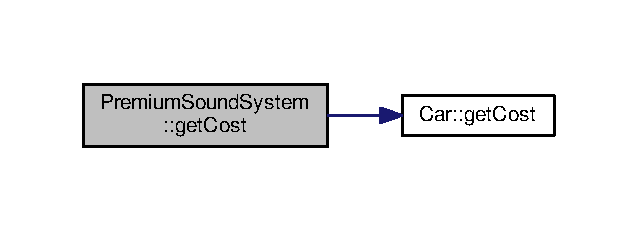
\includegraphics[width=306pt]{classPremiumSoundSystem_ad14f7dae4adfb94572a80199174425af_cgraph}
\end{center}
\end{figure}


\index{Premium\+Sound\+System@{Premium\+Sound\+System}!get\+Description@{get\+Description}}
\index{get\+Description@{get\+Description}!Premium\+Sound\+System@{Premium\+Sound\+System}}
\subsubsection[{\texorpdfstring{get\+Description()}{getDescription()}}]{\setlength{\rightskip}{0pt plus 5cm}string Premium\+Sound\+System\+::get\+Description (
\begin{DoxyParamCaption}
{}
\end{DoxyParamCaption}
)\hspace{0.3cm}{\ttfamily [inline]}, {\ttfamily [virtual]}}\hypertarget{classPremiumSoundSystem_a11267003bbf024bf19b811b0b28b22c1}{}\label{classPremiumSoundSystem_a11267003bbf024bf19b811b0b28b22c1}


Implements \hyperlink{classOptionsDecorator_a620341446534468345792530d454f76c}{Options\+Decorator}.


\begin{DoxyCode}
92                 \{
93                         \textcolor{keywordflow}{return} \hyperlink{classPremiumSoundSystem_a441bc8062467c6c45cd47bca4b8950dd}{\_b}->\hyperlink{classCar_a0d2f99b108e72e2a44360b38f16bbb46}{getDescription}() + \textcolor{stringliteral}{", PremiumSoundSystem"};
94                 \}
\end{DoxyCode}


Here is the call graph for this function\+:
\nopagebreak
\begin{figure}[H]
\begin{center}
\leavevmode
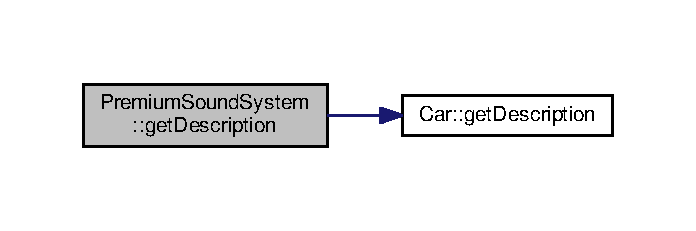
\includegraphics[width=334pt]{classPremiumSoundSystem_a11267003bbf024bf19b811b0b28b22c1_cgraph}
\end{center}
\end{figure}




\subsection{Member Data Documentation}
\index{Premium\+Sound\+System@{Premium\+Sound\+System}!\+\_\+b@{\+\_\+b}}
\index{\+\_\+b@{\+\_\+b}!Premium\+Sound\+System@{Premium\+Sound\+System}}
\subsubsection[{\texorpdfstring{\+\_\+b}{_b}}]{\setlength{\rightskip}{0pt plus 5cm}{\bf Car}$\ast$ Premium\+Sound\+System\+::\+\_\+b\hspace{0.3cm}{\ttfamily [private]}}\hypertarget{classPremiumSoundSystem_a441bc8062467c6c45cd47bca4b8950dd}{}\label{classPremiumSoundSystem_a441bc8062467c6c45cd47bca4b8950dd}


The documentation for this class was generated from the following file\+:\begin{DoxyCompactItemize}
\item 
\hyperlink{Decorator_8cpp}{Decorator.\+cpp}\end{DoxyCompactItemize}

\chapter{File Documentation}
\hypertarget{Decorator_8cpp}{}\section{Decorator.\+cpp File Reference}
\label{Decorator_8cpp}\index{Decorator.\+cpp@{Decorator.\+cpp}}
{\ttfamily \#include $<$string$>$}\\*
{\ttfamily \#include $<$iostream$>$}\\*
Include dependency graph for Decorator.\+cpp\+:
\nopagebreak
\begin{figure}[H]
\begin{center}
\leavevmode
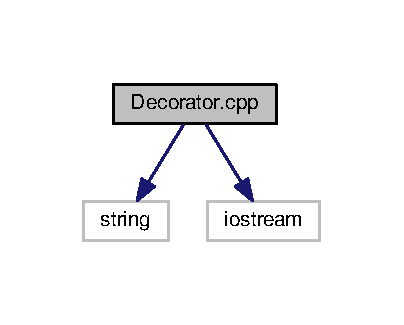
\includegraphics[width=194pt]{Decorator_8cpp__incl}
\end{center}
\end{figure}
\subsection*{Classes}
\begin{DoxyCompactItemize}
\item 
class \hyperlink{classCar}{Car}
\item 
class \hyperlink{classOptionsDecorator}{Options\+Decorator}
\item 
class \hyperlink{classCarModel1}{Car\+Model1}
\item 
class \hyperlink{classNavigation}{Navigation}
\item 
class \hyperlink{classPremiumSoundSystem}{Premium\+Sound\+System}
\item 
class \hyperlink{classManualTransmission}{Manual\+Transmission}
\end{DoxyCompactItemize}
\subsection*{Functions}
\begin{DoxyCompactItemize}
\item 
int \hyperlink{Decorator_8cpp_ae66f6b31b5ad750f1fe042a706a4e3d4}{main} ()
\end{DoxyCompactItemize}


\subsection{Function Documentation}
\index{Decorator.\+cpp@{Decorator.\+cpp}!main@{main}}
\index{main@{main}!Decorator.\+cpp@{Decorator.\+cpp}}
\subsubsection[{\texorpdfstring{main()}{main()}}]{\setlength{\rightskip}{0pt plus 5cm}int main (
\begin{DoxyParamCaption}
{}
\end{DoxyParamCaption}
)}\hypertarget{Decorator_8cpp_ae66f6b31b5ad750f1fe042a706a4e3d4}{}\label{Decorator_8cpp_ae66f6b31b5ad750f1fe042a706a4e3d4}

\begin{DoxyCode}
132 \{
133         \textcolor{comment}{//Create our Car that we want to buy}
134         \hyperlink{classCar}{Car} *b = \textcolor{keyword}{new} \hyperlink{classCarModel1}{CarModel1}();
135 
136         cout << \textcolor{stringliteral}{"Base model of "} << b->\hyperlink{classCar_a0d2f99b108e72e2a44360b38f16bbb46}{getDescription}() << \textcolor{stringliteral}{" costs $"} << b->
      \hyperlink{classCar_a7498766d25f7d4f15272f8055dd698f4}{getCost}() << \textcolor{stringliteral}{"\(\backslash\)n"};  
137             
138         \textcolor{comment}{//Who wants base model let's add some more features}
139             
140         b = \textcolor{keyword}{new} \hyperlink{classNavigation}{Navigation}(b);
141         cout << b->\hyperlink{classCar_a0d2f99b108e72e2a44360b38f16bbb46}{getDescription}() << \textcolor{stringliteral}{" will cost you $"} << b->
      \hyperlink{classCar_a7498766d25f7d4f15272f8055dd698f4}{getCost}() << \textcolor{stringliteral}{"\(\backslash\)n"};
142         b = \textcolor{keyword}{new} \hyperlink{classPremiumSoundSystem}{PremiumSoundSystem}(b);
143         b = \textcolor{keyword}{new} \hyperlink{classManualTransmission}{ManualTransmission}(b);
144         cout << b->\hyperlink{classCar_a0d2f99b108e72e2a44360b38f16bbb46}{getDescription}() << \textcolor{stringliteral}{" will cost you $"} << b->
      \hyperlink{classCar_a7498766d25f7d4f15272f8055dd698f4}{getCost}() << \textcolor{stringliteral}{"\(\backslash\)n"};
145 
146         \textcolor{comment}{// WARNING! Here we leak the CarModel1, Navigation and PremiumSoundSystem objects!}
147         \textcolor{comment}{// Either we delete them explicitly or rewrite the Decorators to take }
148         \textcolor{comment}{// ownership and delete their Cars when destroyed.}
149         \textcolor{keyword}{delete} b;
150 
151         \textcolor{keywordflow}{return} 0;
152 \}\end{DoxyCode}


Here is the call graph for this function\+:
\nopagebreak
\begin{figure}[H]
\begin{center}
\leavevmode
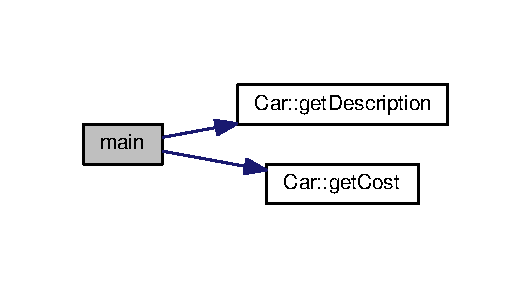
\includegraphics[width=255pt]{Decorator_8cpp_ae66f6b31b5ad750f1fe042a706a4e3d4_cgraph}
\end{center}
\end{figure}



%--- End generated contents ---

% Index
\backmatter
\newpage
\phantomsection
\clearemptydoublepage
\addcontentsline{toc}{chapter}{Index}
\printindex

\end{document}
